\section{并行思路与方法}

在这一章,将按照并行加载数据、不同的并行方式这两个角度来阐述并行算法的思路与设计方法。
并行训练模型可分为两种:数据并行和模型并行。数据并行是指:多个GPU使用相同的模型副本,但采用
不同的数据进行训练\cite{part};模型并行是指:当模型过大时,多个GPU使用相同的数据分别训练模型的不同部分。因实验选用
的GPU足以容纳模型和数据,因此采用数据并行的形式来加速网络的执行。

\subsection{并行加载数据}

在加载数据时,可以使用多进程来加载数据。不使用多线程的目的是:python的多线程因为GIL(Global Interpreter Lock)
的存在,只能在单核运行。不能发挥多核处理器的优势,因此只适合I/O型任务,不适合密集计算型任务。

首先以torch.utils.data.Dataset为父类,创建一个加载数据集的子类:MiniImagenet。在MiniImagenet中,
设置\_\_getitem\_\_方法来支持数据集的切片访问,即批量加载数据。

在训练阶段,实例化加载数据集的类,得到一个实例对象。在torch.utils.data.D\-ataLoader中传入
实例对象来加载数据,并设置其他参数来提升加载数据的速度和数量。设置num\_workers=8可以使用8进程来加载数据,
设置batch\_size=batchsz对应MiniImagenet类的\_\_getitem\_\_切片访问,即一次获取的训练数据的大小。

在创建num\_workers个进程之后,多个进程共享一份数据集,将指定batch(一批待加载的目标数据)分配给指定worker(一个进程),
worker将对应batch的数据加载进内存。因此增大num\_workers的数量,内存的占用率也会增加。
在第一个batch的数据加载完成后,会等待主进程将该batch取走并汇总,而后此worker开始加载下一个batch,不断迭代。

主进程采集完最后一个worker的数据后,此时需要返回并采集第一个worker加载的第二个batch。
如果第一个worker此时没有加载完,主线程将阻塞等待当前worker的数据加载完毕。
最后所有数据加载完毕后,汇总到一起供用户使用。

当num\_worker设置的很大时,优点时可以快速的寻找目标batch;缺点是内存开销大,也加重了CPU维护进程的开销,
如创建、初始化、通信、分配任务、接受任务反馈和销毁进程等\cite{process}。
num\_workers的经验设置值是服务器的CPU核心数,如果CPU性能强大且内存充足,可以设置为较大的数值。

\subsection{DataParallel并行方式}

DataParallel并行方式实现较为简单。首先将模型放到主GPU中,一般是GPU-0;而后将模型复制得到副本,将模型
副本放到另外的$n$张GPU中,将输入的batchsz大小的数据平均分为$n$份依次作为每个模型副本的输入。因此
要求batchsz的大小要大于GPU的数量,否则数据无法分配,会导致有的模型副本得不到数据。

每个模型副本
独立的进行前向计算,得到各自的loss值。在$n$个GPU完成计算后,将loss汇总到GPU-0中,由GPU-0中的模型进行反向传播和
更新参数。更新好参数后,由GPU-0将参数分发至其他$n$个GPU卡,开始新一轮的计算。
DataParallel并行结构示意图如图\ref{fig:dp-stru}所示:

\begin{figure}[h]
    \centering
    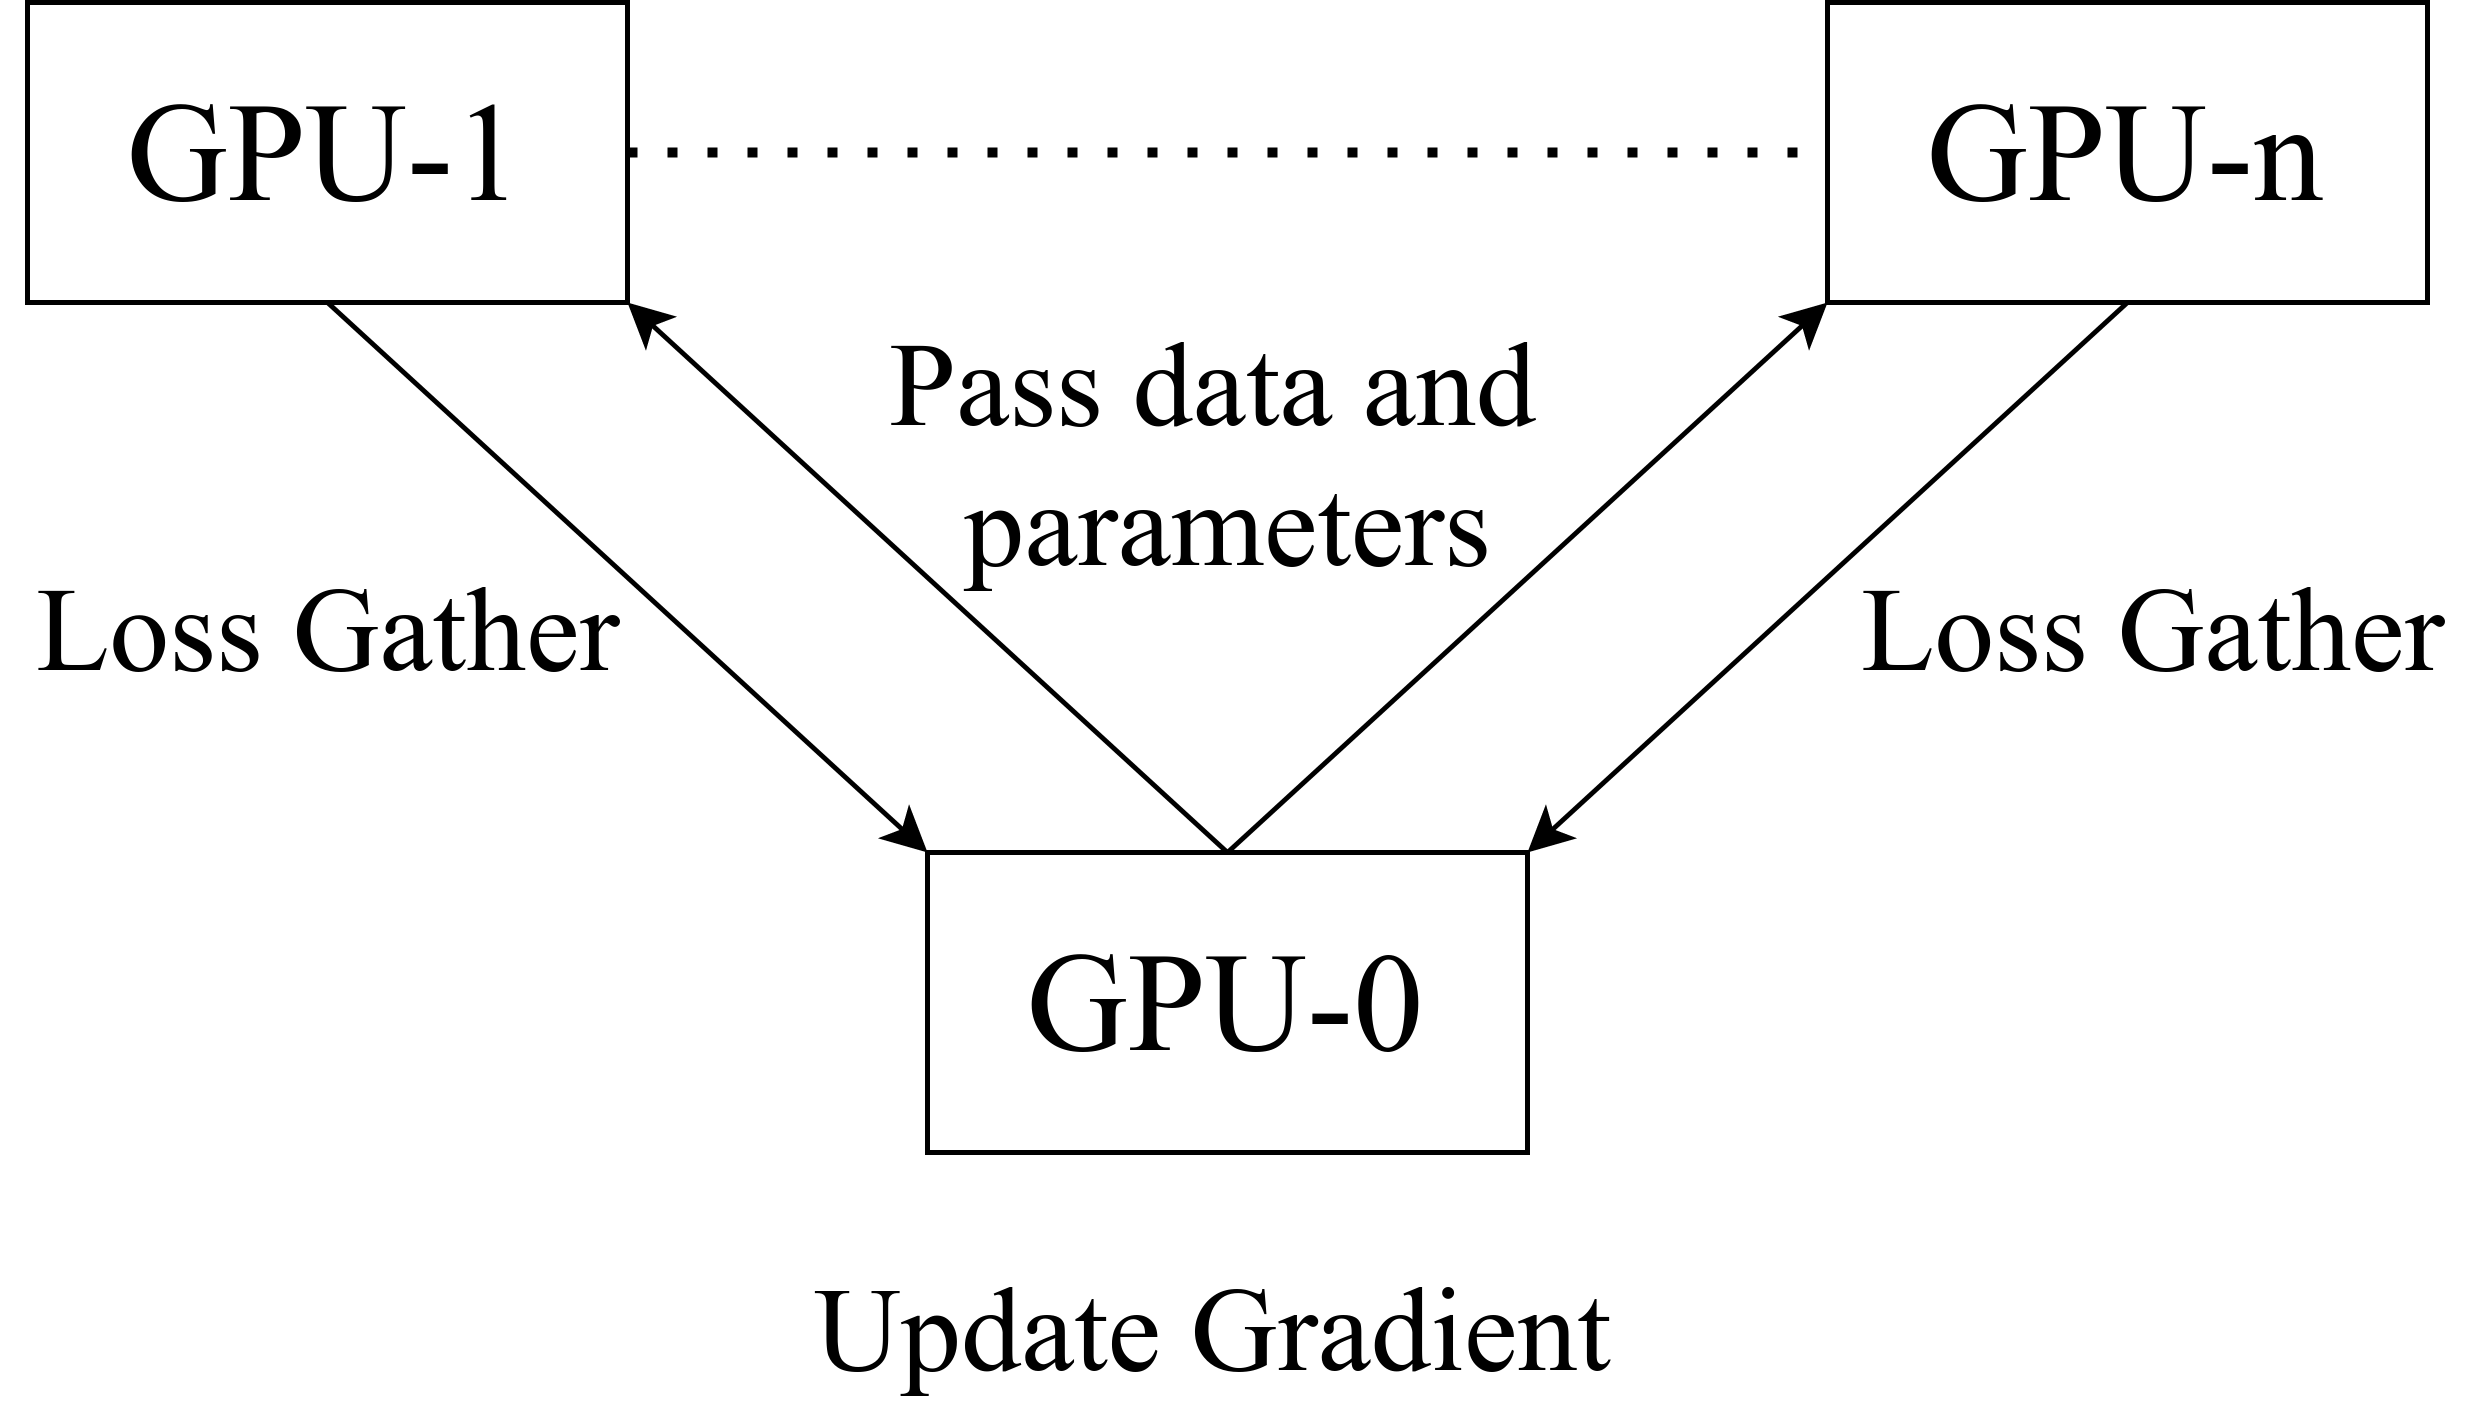
\includegraphics[scale=0.15]{figure/dp-structure.png}
    \caption{DataParallel并行结构示意图}
    \label{fig:dp-stru}
\end{figure}

DataParallel基于单进程多线程实现,因为python的多线程无法利用多核处理器,只能在单核上进行任务调度和参数更新的通信,
所以此种方式并行效率较低,且0号卡负担较大。

\subsection{DistributedDataParallel并行方式}

DistributedDataParallel并行方式实现较为复杂,且相对于DataParallel需要更大的显存空间。
DistributedDataParallel使用的进程数量一般和GPU数量相等,对每个进程创建一个DistributedDataParallel实例,
通过进程通信来同步梯度,通信方式为AllReduce\cite{ar}。

在任务初始化阶段,即并行程序执行之前首先要创建通信群组,通信群组中的每一个进程创建一个DistributedDataParallel实例
。DistributedDataParallel通过rank0(进程ID)将当前
模型的结构和参数等状态通过广播通信的形式发送到进程组的所有进程中,确保其他进程中的模型副本和当前模型保持一致。
而后,每个进程创建一个本地的Reducer,用于反向传播阶段同步参数的梯度。因此相比于DataParallel,
DistributedDataParallel需要更大的显存容量。
为了提升通信效率,Reducer将参数放到多个桶中,每次以桶为单位进行通信\cite{bucket}。

参数需要额外附加unready和ready两种状态,默认为unready状态。
若参数在反向传播阶段计算了梯度,则参数由unready状态变为ready状态,表示这个参数可以同步到其他模型;否则保持unready状态。
当模型完成一次训练后,参数由ready状态变为unready状态,为下一次训练做准备。

因为在反向传播阶段,DistributedDataParallel只会等待unready状态的参数更新,
所以在前向计算阶段首先要分析计算图,将不进行梯度更新的参数状态永久设为ready状态,防止这些参数影响反向传播。
DistributedDataParallel在获取输入数据后,
将输入数据分发到每个GPU中,模型副本开始前向计算得到各自的loss值,而后开始反向传播。

DistributedDataParallel在初始化阶段会为每一个可求导的参数申请一个自动求导的钩子,来发射同步梯度的信号。
在反向传播阶段,当一个参数计算梯度后会为ready状态,对应梯度的钩子就会发射信号,
DistributedDataParallel会标记该参数的状态,表示该参数的梯度可以用于同步。
当一个桶内的参数全部由unready状态变为ready状态后,
Reducer通过AllReduce的通信方式来更新桶内的参数,来计算所有模型副本中参数梯度的平均值。
以4个GPU为例,其AllReduce通信方式如图\ref{fig:allre}所示。

\begin{figure}[h]
    \centering
    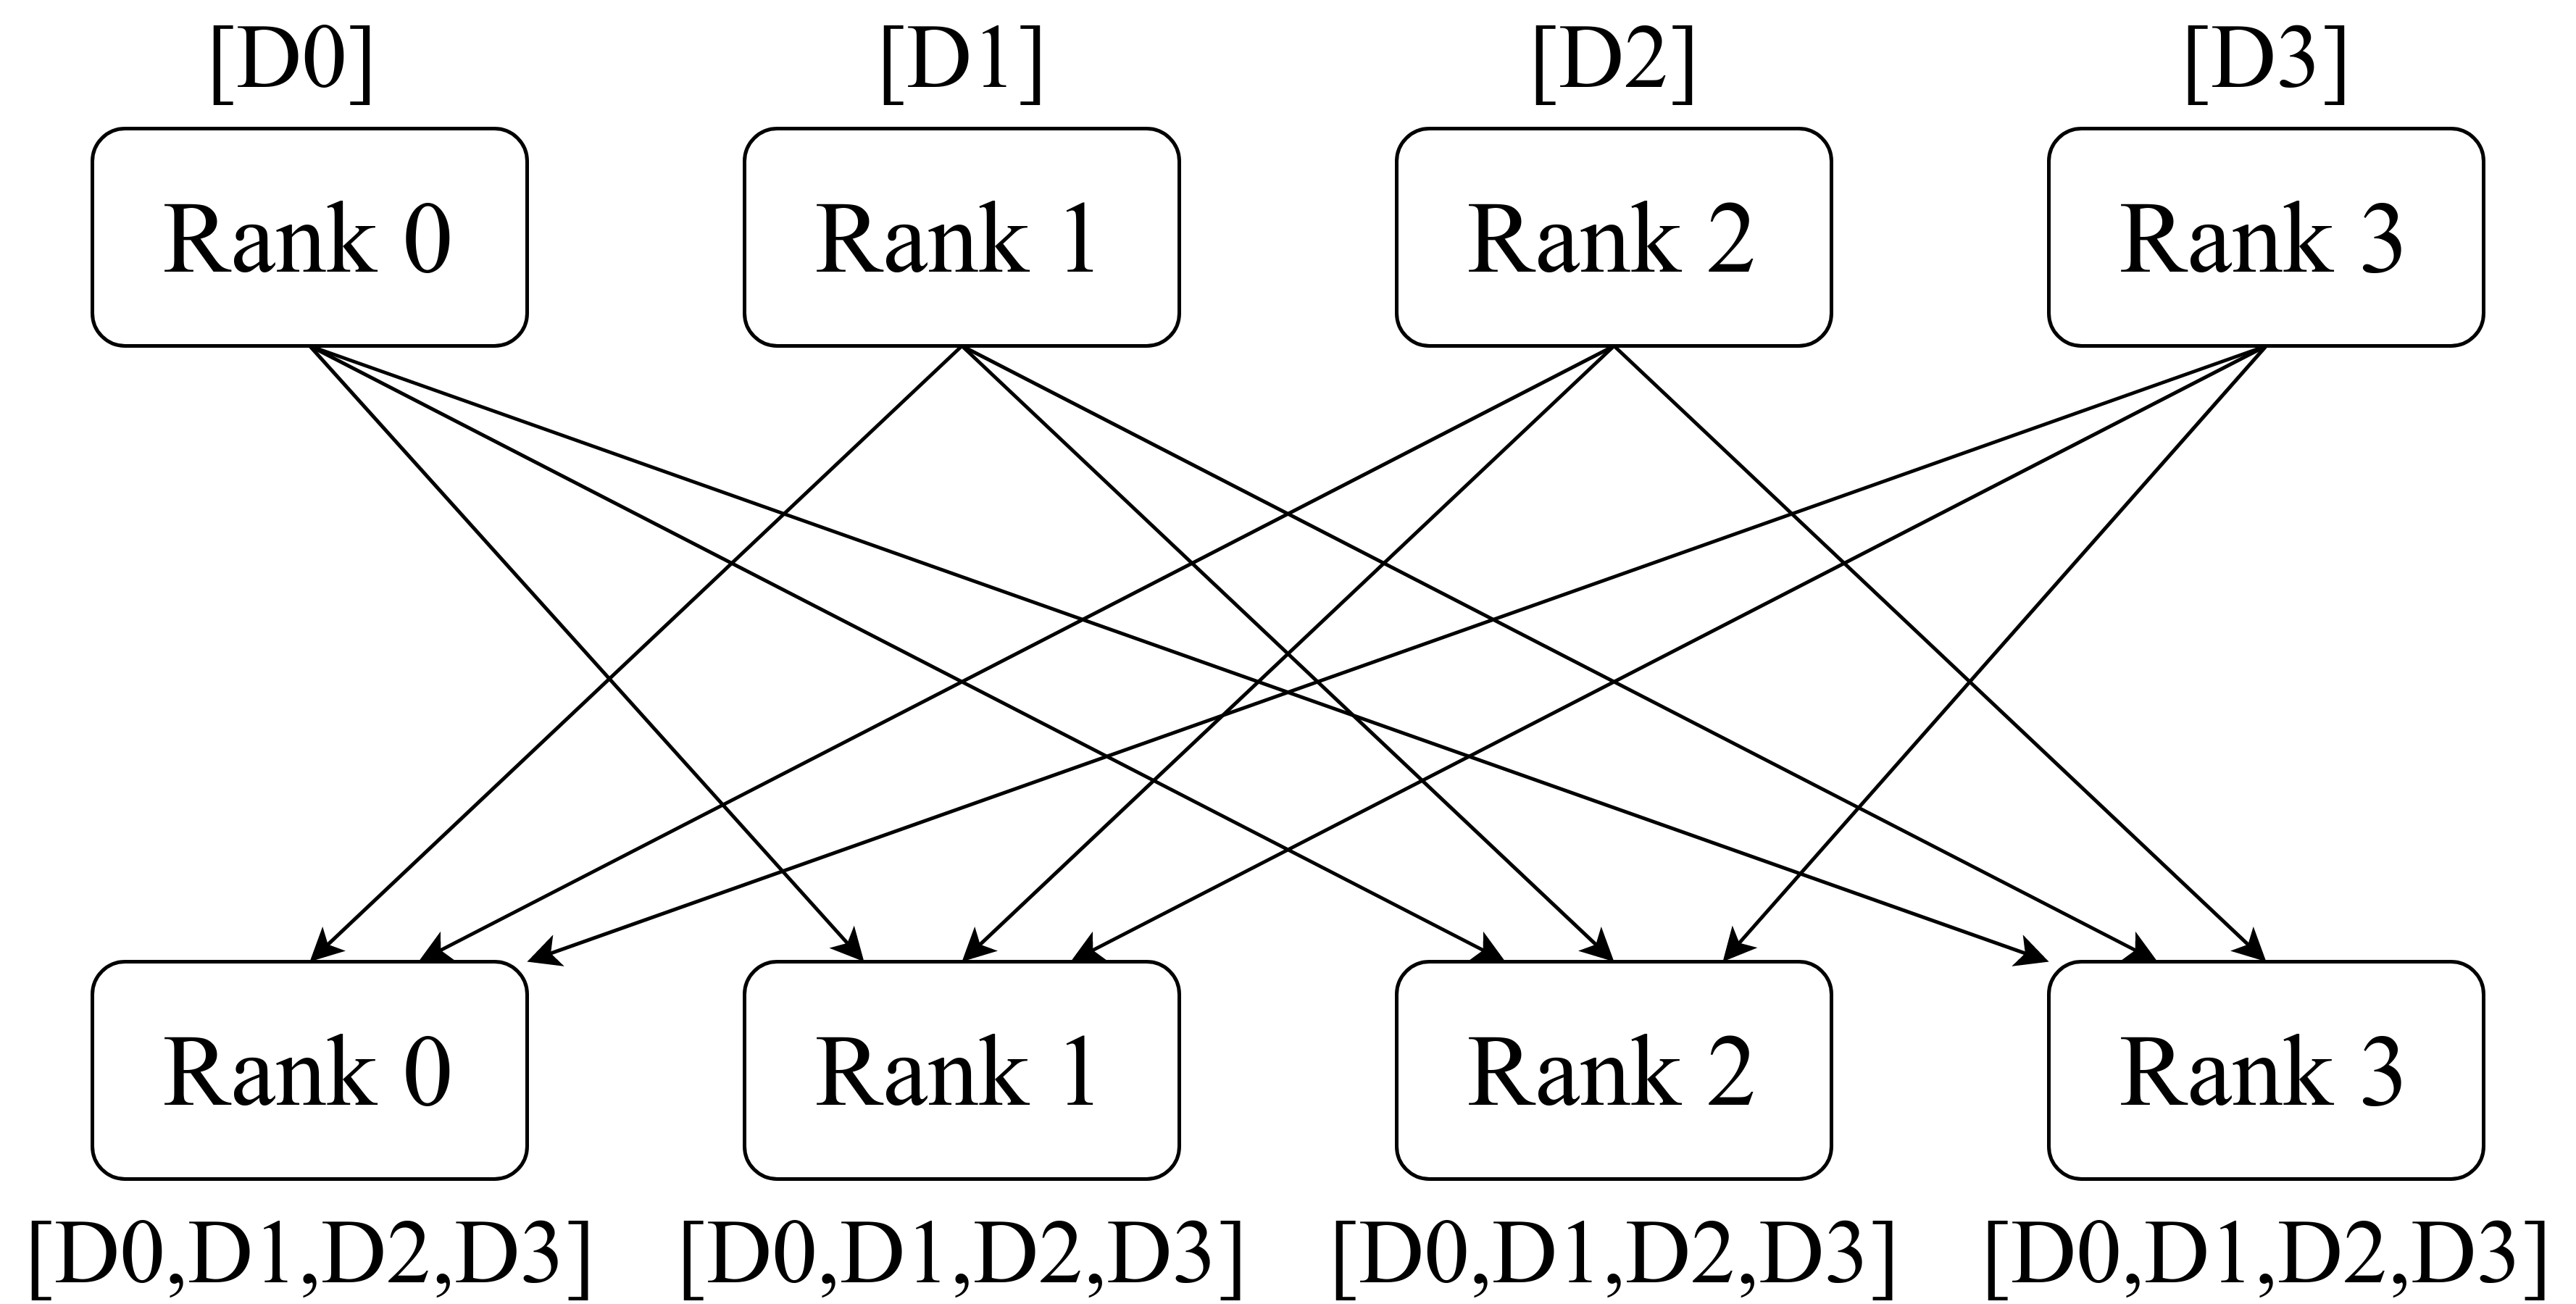
\includegraphics[scale=0.1]{figure/all-reduce.png}
    \caption{AllReduce通信方法示意图}
    \label{fig:allre}
\end{figure}

在图\ref{fig:allre}中,
rank0将自己模型副本的梯度D0发送给rank1,rank2和rank3,其他进程同理。因此在AllReduce
通信后,所有的模型副本的梯度值保持一致。

当所有的桶更新完毕后,Reducer会阻塞等待
AllReduce的所有操作结束,如重新将参数设为unready状态。因为所有模型副本的梯度值相同,
所以在梯度更新阶段,只需更新本卡中的模型参数。因为所有的模型副本来自相同的初始状态,且具有相同的平均梯度值,
所以在梯度更新后所的模型副本状态都会保持一致,以此来实现并行。

\subsection{并行方式的对比}

DataParallel和DistributedDataParallel都属于数据并行的方法,在分析完各自的实现原理后,可以得到
二者的对比。对比情况如表\ref{tab:com}所示:

\begin{table}[h]
    \centering
    \caption{DataParallel与DistributedDataParallel对比}
    \begin{tabular}{>{\centering\arraybackslash}p{5em}>{\centering\arraybackslash}p{12em}>{\centering\arraybackslash}p{13em}}
    \toprule
    { } & DataParallel & DistributedParallel \\ \midrule
    机器支持 & 只支持单机 & 可支持多机 \\
    模型支持 & 不支持拆分模型 & 可以将模型放到多张GPU中 \\
    通信方式 & scatter input 和 gather output & scatter input 和 AllReduce \\
    并行支持 & 只支持数据并行 & 支持数据并行和模型并行 \\
    进程与线程 & 单进程、多线程 & 多进程 \\
    \bottomrule
    \end{tabular}
    \label{tab:com}
\end{table}